% Options for packages loaded elsewhere
\PassOptionsToPackage{unicode}{hyperref}
\PassOptionsToPackage{hyphens}{url}
\PassOptionsToPackage{dvipsnames,svgnames,x11names}{xcolor}
%
\documentclass[
  letterpaper,
  DIV=11,
  numbers=noendperiod]{scrartcl}

\usepackage{amsmath,amssymb}
\usepackage{iftex}
\ifPDFTeX
  \usepackage[T1]{fontenc}
  \usepackage[utf8]{inputenc}
  \usepackage{textcomp} % provide euro and other symbols
\else % if luatex or xetex
  \usepackage{unicode-math}
  \defaultfontfeatures{Scale=MatchLowercase}
  \defaultfontfeatures[\rmfamily]{Ligatures=TeX,Scale=1}
\fi
\usepackage{lmodern}
\ifPDFTeX\else  
    % xetex/luatex font selection
\fi
% Use upquote if available, for straight quotes in verbatim environments
\IfFileExists{upquote.sty}{\usepackage{upquote}}{}
\IfFileExists{microtype.sty}{% use microtype if available
  \usepackage[]{microtype}
  \UseMicrotypeSet[protrusion]{basicmath} % disable protrusion for tt fonts
}{}
\makeatletter
\@ifundefined{KOMAClassName}{% if non-KOMA class
  \IfFileExists{parskip.sty}{%
    \usepackage{parskip}
  }{% else
    \setlength{\parindent}{0pt}
    \setlength{\parskip}{6pt plus 2pt minus 1pt}}
}{% if KOMA class
  \KOMAoptions{parskip=half}}
\makeatother
\usepackage{xcolor}
\setlength{\emergencystretch}{3em} % prevent overfull lines
\setcounter{secnumdepth}{5}
% Make \paragraph and \subparagraph free-standing
\ifx\paragraph\undefined\else
  \let\oldparagraph\paragraph
  \renewcommand{\paragraph}[1]{\oldparagraph{#1}\mbox{}}
\fi
\ifx\subparagraph\undefined\else
  \let\oldsubparagraph\subparagraph
  \renewcommand{\subparagraph}[1]{\oldsubparagraph{#1}\mbox{}}
\fi

\usepackage{color}
\usepackage{fancyvrb}
\newcommand{\VerbBar}{|}
\newcommand{\VERB}{\Verb[commandchars=\\\{\}]}
\DefineVerbatimEnvironment{Highlighting}{Verbatim}{commandchars=\\\{\}}
% Add ',fontsize=\small' for more characters per line
\usepackage{framed}
\definecolor{shadecolor}{RGB}{241,243,245}
\newenvironment{Shaded}{\begin{snugshade}}{\end{snugshade}}
\newcommand{\AlertTok}[1]{\textcolor[rgb]{0.68,0.00,0.00}{#1}}
\newcommand{\AnnotationTok}[1]{\textcolor[rgb]{0.37,0.37,0.37}{#1}}
\newcommand{\AttributeTok}[1]{\textcolor[rgb]{0.40,0.45,0.13}{#1}}
\newcommand{\BaseNTok}[1]{\textcolor[rgb]{0.68,0.00,0.00}{#1}}
\newcommand{\BuiltInTok}[1]{\textcolor[rgb]{0.00,0.23,0.31}{#1}}
\newcommand{\CharTok}[1]{\textcolor[rgb]{0.13,0.47,0.30}{#1}}
\newcommand{\CommentTok}[1]{\textcolor[rgb]{0.37,0.37,0.37}{#1}}
\newcommand{\CommentVarTok}[1]{\textcolor[rgb]{0.37,0.37,0.37}{\textit{#1}}}
\newcommand{\ConstantTok}[1]{\textcolor[rgb]{0.56,0.35,0.01}{#1}}
\newcommand{\ControlFlowTok}[1]{\textcolor[rgb]{0.00,0.23,0.31}{#1}}
\newcommand{\DataTypeTok}[1]{\textcolor[rgb]{0.68,0.00,0.00}{#1}}
\newcommand{\DecValTok}[1]{\textcolor[rgb]{0.68,0.00,0.00}{#1}}
\newcommand{\DocumentationTok}[1]{\textcolor[rgb]{0.37,0.37,0.37}{\textit{#1}}}
\newcommand{\ErrorTok}[1]{\textcolor[rgb]{0.68,0.00,0.00}{#1}}
\newcommand{\ExtensionTok}[1]{\textcolor[rgb]{0.00,0.23,0.31}{#1}}
\newcommand{\FloatTok}[1]{\textcolor[rgb]{0.68,0.00,0.00}{#1}}
\newcommand{\FunctionTok}[1]{\textcolor[rgb]{0.28,0.35,0.67}{#1}}
\newcommand{\ImportTok}[1]{\textcolor[rgb]{0.00,0.46,0.62}{#1}}
\newcommand{\InformationTok}[1]{\textcolor[rgb]{0.37,0.37,0.37}{#1}}
\newcommand{\KeywordTok}[1]{\textcolor[rgb]{0.00,0.23,0.31}{#1}}
\newcommand{\NormalTok}[1]{\textcolor[rgb]{0.00,0.23,0.31}{#1}}
\newcommand{\OperatorTok}[1]{\textcolor[rgb]{0.37,0.37,0.37}{#1}}
\newcommand{\OtherTok}[1]{\textcolor[rgb]{0.00,0.23,0.31}{#1}}
\newcommand{\PreprocessorTok}[1]{\textcolor[rgb]{0.68,0.00,0.00}{#1}}
\newcommand{\RegionMarkerTok}[1]{\textcolor[rgb]{0.00,0.23,0.31}{#1}}
\newcommand{\SpecialCharTok}[1]{\textcolor[rgb]{0.37,0.37,0.37}{#1}}
\newcommand{\SpecialStringTok}[1]{\textcolor[rgb]{0.13,0.47,0.30}{#1}}
\newcommand{\StringTok}[1]{\textcolor[rgb]{0.13,0.47,0.30}{#1}}
\newcommand{\VariableTok}[1]{\textcolor[rgb]{0.07,0.07,0.07}{#1}}
\newcommand{\VerbatimStringTok}[1]{\textcolor[rgb]{0.13,0.47,0.30}{#1}}
\newcommand{\WarningTok}[1]{\textcolor[rgb]{0.37,0.37,0.37}{\textit{#1}}}

\providecommand{\tightlist}{%
  \setlength{\itemsep}{0pt}\setlength{\parskip}{0pt}}\usepackage{longtable,booktabs,array}
\usepackage{calc} % for calculating minipage widths
% Correct order of tables after \paragraph or \subparagraph
\usepackage{etoolbox}
\makeatletter
\patchcmd\longtable{\par}{\if@noskipsec\mbox{}\fi\par}{}{}
\makeatother
% Allow footnotes in longtable head/foot
\IfFileExists{footnotehyper.sty}{\usepackage{footnotehyper}}{\usepackage{footnote}}
\makesavenoteenv{longtable}
\usepackage{graphicx}
\makeatletter
\def\maxwidth{\ifdim\Gin@nat@width>\linewidth\linewidth\else\Gin@nat@width\fi}
\def\maxheight{\ifdim\Gin@nat@height>\textheight\textheight\else\Gin@nat@height\fi}
\makeatother
% Scale images if necessary, so that they will not overflow the page
% margins by default, and it is still possible to overwrite the defaults
% using explicit options in \includegraphics[width, height, ...]{}
\setkeys{Gin}{width=\maxwidth,height=\maxheight,keepaspectratio}
% Set default figure placement to htbp
\makeatletter
\def\fps@figure{htbp}
\makeatother

% load packages
\usepackage{geometry}
\usepackage{xcolor}
\usepackage{eso-pic}
\usepackage{fancyhdr}
\usepackage{sectsty}
\usepackage{fontspec}
\usepackage{titlesec}

%% Set page size with a wider right margin
\geometry{a4paper, total={170mm,257mm}, left=20mm, top=20mm, bottom=20mm, right=50mm}

%% Let's define some colours
\definecolor{uniblue}{HTML}{003865}
\definecolor{burgundy}{HTML}{7D2239}
\definecolor{cobalt}{HTML}{005C8A}
\definecolor{lavender}{HTML}{5B4D94}
\definecolor{leaf}{HTML}{006630}
\definecolor{moss}{HTML}{385A4F}
\definecolor{pillarbox}{HTML}{B30C00}
\definecolor{rust}{HTML}{9A3A06}
\definecolor{sandstone}{HTML}{52473B}
\definecolor{skyblue}{HTML}{005398}
\definecolor{slate}{HTML}{4F5961}
\definecolor{thistle}{HTML}{951272}

%\definecolor{light}{HTML}{E6E6FA} % original from template - redefined below as uni blue at 10 percent:
\colorlet{light}{uniblue!10}
%\definecolor{highlight}{HTML}{800080} % original from template - redefined below as uni's skyblue:
\colorlet{highlight}{skyblue}
%\definecolor{dark}{HTML}{330033} % original from template - redefined below as uni blue at 100 percent:
\colorlet{dark}{uniblue}

%% Let's add the border on the right hand side 
\AddToShipoutPicture{% 
    \AtPageLowerLeft{% 
        \put(\LenToUnit{\dimexpr\paperwidth-3cm},0){% 
            \color{light}\rule{3cm}{\LenToUnit\paperheight}%
          }%
     }%
     % logo
    \AtPageLowerLeft{% start the bar at the bottom right of the page
        \put(\LenToUnit{\dimexpr\paperwidth-2.25cm},27.2cm){% move it to the top right
            \color{light}
\includegraphics[width=2.25cm]{_extensions/nrennie/PrettyPDF/uni_logo_boxed.jpg}
          }%
     }%
}

%% Style the page number
\fancypagestyle{mystyle}{
  \fancyhf{}
  \renewcommand\headrulewidth{0pt}
  \fancyfoot[R]{\thepage}
  \fancyfootoffset{3.5cm}
}
\setlength{\footskip}{20pt}

%% style the chapter/section fonts
\chapterfont{\color{uniblue}\fontsize{20}{16.8}\selectfont}
\sectionfont{\color{uniblue}\fontsize{20}{16.8}\selectfont}
\subsectionfont{\color{skyblue}\fontsize{14}{16.8}\selectfont}
\titleformat{\subsection}
  {\color{uniblue!90}\sffamily\Large\bfseries}{\thesubsection}{1em}{}[{\titlerule[0.8pt]}]
\subsubsectionfont{\color{cobalt}}

\renewcommand\thesection{\color{slate}\arabic{section}}
  
% left align title
\makeatletter
\renewcommand{\maketitle}{\bgroup\setlength{\parindent}{0pt}
\begin{flushleft}
  {\color{uniblue}\sffamily\huge\textbf{\@title}} \vspace{0.3cm} \newline
  {\Large {\@subtitle}} \newline
  \@author
\end{flushleft}\egroup
}
\makeatother

%% Use some custom fonts
\setsansfont{Ubuntu}[
    Path=_extensions/nrennie/PrettyPDF/Ubuntu/,
    Scale=0.9,
    Extension = .ttf,
    UprightFont=*-Regular,
    BoldFont=*-Bold,
    ItalicFont=*-Italic,
    ]

\setmainfont{Ubuntu}[
    Path=_extensions/nrennie/PrettyPDF/Ubuntu/,
    Scale=0.9,
    Extension = .ttf,
    UprightFont=*-Regular,
    BoldFont=*-Bold,
    ItalicFont=*-Italic,
    ]
\KOMAoption{captions}{tableheading}
\makeatletter
\@ifpackageloaded{tcolorbox}{}{\usepackage[skins,breakable]{tcolorbox}}
\@ifpackageloaded{fontawesome5}{}{\usepackage{fontawesome5}}
\definecolor{quarto-callout-color}{HTML}{909090}
\definecolor{quarto-callout-note-color}{HTML}{0758E5}
\definecolor{quarto-callout-important-color}{HTML}{CC1914}
\definecolor{quarto-callout-warning-color}{HTML}{EB9113}
\definecolor{quarto-callout-tip-color}{HTML}{00A047}
\definecolor{quarto-callout-caution-color}{HTML}{FC5300}
\definecolor{quarto-callout-color-frame}{HTML}{acacac}
\definecolor{quarto-callout-note-color-frame}{HTML}{4582ec}
\definecolor{quarto-callout-important-color-frame}{HTML}{d9534f}
\definecolor{quarto-callout-warning-color-frame}{HTML}{f0ad4e}
\definecolor{quarto-callout-tip-color-frame}{HTML}{02b875}
\definecolor{quarto-callout-caution-color-frame}{HTML}{fd7e14}
\makeatother
\makeatletter
\@ifpackageloaded{caption}{}{\usepackage{caption}}
\AtBeginDocument{%
\ifdefined\contentsname
  \renewcommand*\contentsname{Table of contents}
\else
  \newcommand\contentsname{Table of contents}
\fi
\ifdefined\listfigurename
  \renewcommand*\listfigurename{List of Figures}
\else
  \newcommand\listfigurename{List of Figures}
\fi
\ifdefined\listtablename
  \renewcommand*\listtablename{List of Tables}
\else
  \newcommand\listtablename{List of Tables}
\fi
\ifdefined\figurename
  \renewcommand*\figurename{Figure}
\else
  \newcommand\figurename{Figure}
\fi
\ifdefined\tablename
  \renewcommand*\tablename{Table}
\else
  \newcommand\tablename{Table}
\fi
}
\@ifpackageloaded{float}{}{\usepackage{float}}
\floatstyle{ruled}
\@ifundefined{c@chapter}{\newfloat{codelisting}{h}{lop}}{\newfloat{codelisting}{h}{lop}[chapter]}
\floatname{codelisting}{Listing}
\newcommand*\listoflistings{\listof{codelisting}{List of Listings}}
\makeatother
\makeatletter
\makeatother
\makeatletter
\@ifpackageloaded{caption}{}{\usepackage{caption}}
\@ifpackageloaded{subcaption}{}{\usepackage{subcaption}}
\makeatother
\makeatletter
\@ifpackageloaded{tcolorbox}{}{\usepackage[skins,breakable]{tcolorbox}}
\makeatother
\makeatletter
\@ifundefined{shadecolor}{\definecolor{shadecolor}{rgb}{.97, .97, .97}}{}
\makeatother
\makeatletter
\@ifundefined{codebgcolor}{\definecolor{codebgcolor}{named}{light}}{}
\makeatother
\makeatletter
\ifdefined\Shaded\renewenvironment{Shaded}{\begin{tcolorbox}[boxrule=0pt, colback={codebgcolor}, enhanced, sharp corners, breakable, frame hidden]}{\end{tcolorbox}}\fi
\makeatother
\ifLuaTeX
  \usepackage{selnolig}  % disable illegal ligatures
\fi
\usepackage{bookmark}

\IfFileExists{xurl.sty}{\usepackage{xurl}}{} % add URL line breaks if available
\urlstyle{same} % disable monospaced font for URLs
\hypersetup{
  pdftitle={Collaborative Coding 1},
  colorlinks=true,
  linkcolor={highlight},
  filecolor={Maroon},
  citecolor={Blue},
  urlcolor={highlight},
  pdfcreator={LaTeX via pandoc}}

\title{Collaborative Coding 1}
\author{}
\date{}

\begin{document}
\maketitle

\pagestyle{mystyle}

This week's material is based on the
\href{https://moodle.gla.ac.uk/course/view.php?id=41115}{Version Control
Course} from the School of Mathematics and Statistics from the
University of Glasgow. The content has been reduced to fit the class
structure. However, we do encourage you to take a look and attempt the
full course. Please get in touch if you would like to get access the
full course.

\section{Using Git}\label{using-git}

Version control is used throughout industry and academia as a way of
developing and sharing code. Some people tend to think of version
control as simply being GitHub, but it's important to be aware that
version control is a much more general area and GitHub is just a useful
way of hosting a version control system called Git. An alternative
approach might be more appropriate for your project, thus we recommend
thinking through the needs of your project before committing to one
scheme, however Git/GitHub is often a good choice for version control,
hence why we have created a course around it. GitHub, as a host for Git
repositories, is widely used within both academia and industry.

There is an \textbf{increasing requirement} that graduates must have
this skill and you may even start to see version control in some of your
courses if you are a student. From an academic perspective, there is a
drive for open-access code, data, and research. Releasing your code via
GitHub can help others use your research, increasing its utility and
driving the impact of your work.

\subsection{What is a version control
system}\label{what-is-a-version-control-system}

A Version Control System is a tool that helps keep track of code and
software development projects as they change over time. The idea is to
save snapshots of code at any given time, called \textbf{versions}, to
allow developers to understand how the code was developed and if
necessary revert (go back) to previous versions.

When coding collaboratively researchers or developers can work on the
same code base, keeping individual versions of the code separate from
each other. These different sections are called \textbf{branches}, which
you'll learn about in this course, can later be combined by the system
such that code that has stayed the same remains unchanged and changes
made by each researcher or developer can be combined into one version.

\section{Up and running}\label{up-and-running}

To get up and running you will need to install Git and sign up for a
GitHub account. In this section, we will describe how to install Git on
Mac and Windows and how to link it with your GitHub account.

\subsection{Separate instructions for the command line and GitHub
Desktop}\label{separate-instructions-for-the-command-line-and-github-desktop}

As with any tool, there are multiple ways of interacting with it and
individuals tend to choose the way that works best for them/their
workflow. Two of the most common ways of interacting with git/version
control is either through the command line using the `git' command or
through a graphical user interface (GUI).

To address both needs throughout this course, you can either work
through the examples using the command line or GitHub Desktop - a
popular GUI (or compare both) for using Git. When you see a section that
has a border around it, you can select either `Command-line' or `GitHub
Desktop' at the top, and this will change all sections on the page to
your preferred program.

\subsection{Installation and command-line
usage}\label{installation-and-command-line-usage}

As Git is primarily a developer tool, it may be a little harder to
install than you are used to. Git is a command-line program, however,
you can opt to install a graphical user interface (GUI) for Git such as
GitHub Desktop and avoid having to open a command-line terminal at all
if you don't want to!

If you're familiar with installing command-line tools, GitHub provides a
short guide named Install Git that should get you up and running
quickly.

Below are some additional tips for those needing a bit more guidance.

\subsubsection{For Mac users}\label{for-mac-users}

Git is a command-line tool that is usually already installed on Macs and
can be accessed from the built-in terminal. The Terminal application can
be found by navigating to the \texttt{Applications/Utilities} folder or
searching for `Terminal' in Spotlight.

\subsubsection{For Windows users}\label{for-windows-users}

This Getting Started guide provides a bit more detail on which options
to select during the installation process for the best experience.

After clicking the ``Download Git for Windows'' button you will arrive
at a GitHub Release page, with lots of variations to choose from.

To know which option is right for your system, first, you need to find
out if your computer is 32-bit or 64-bit:

Go to
\texttt{Start\ \textgreater{}\ Settings\ \textgreater{}\ System\ \textgreater{}\ About}.
Check the bit version under
\texttt{Device\ specifications\ \textgreater{}\ System\ type}.

Then choose the \texttt{.exe} file that matches your system:

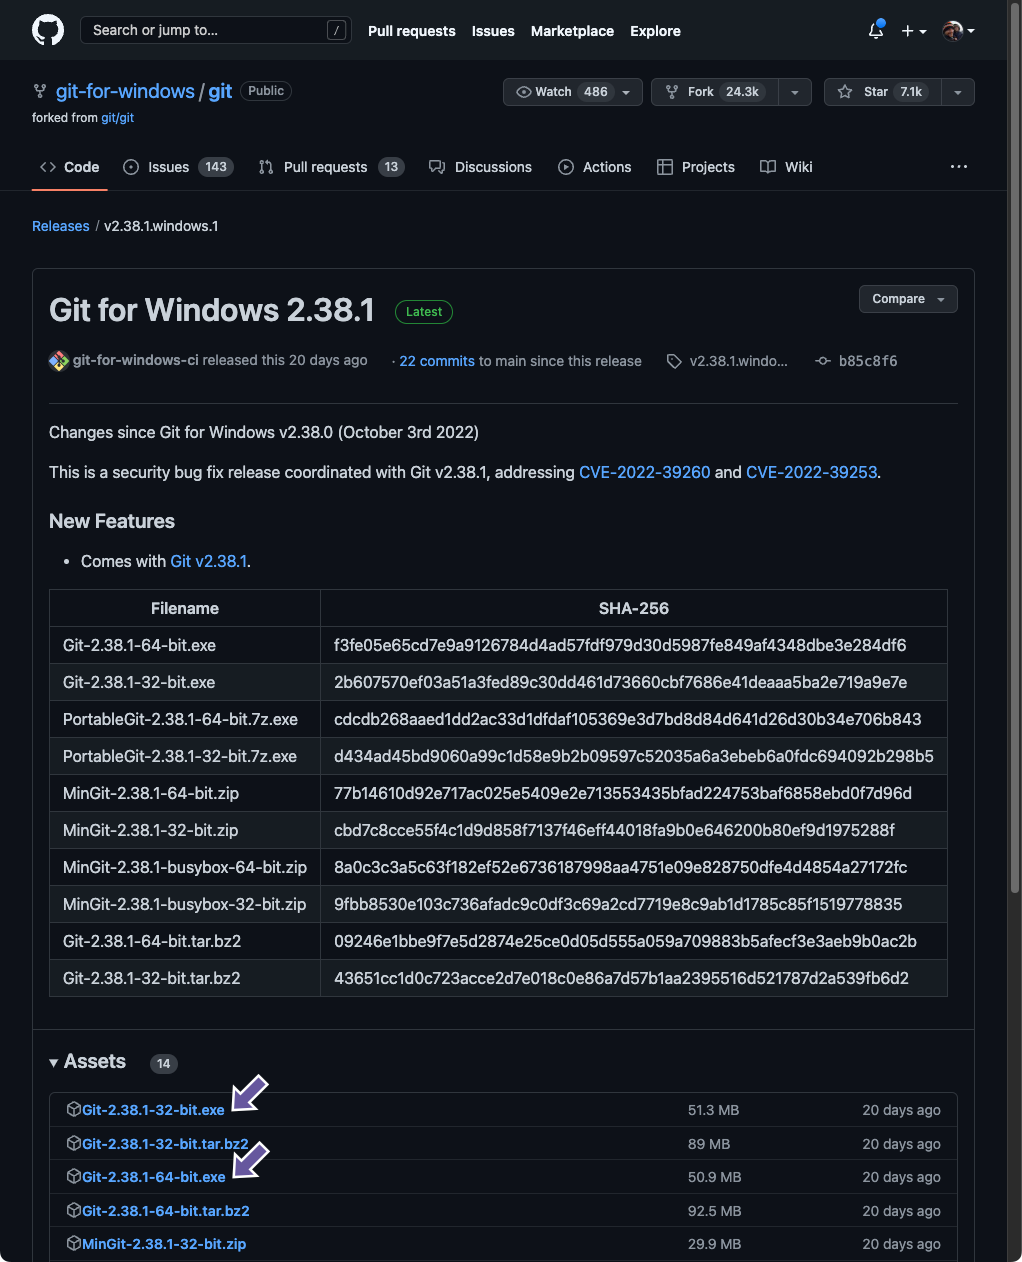
\includegraphics{images/image1.png}

Once installed, it can be accessed from the Git r terminal which comes
included as part of the Git For Windows package. You can find Git r by
opening the Start menu and typing `Git r' into the search bar. However,
if you plan on using a GUI for Git such as GitHub Desktop, you don't
need to open a terminal at all.

\section{Sign up for GitHub}\label{sign-up-for-github}

If you haven't done so already, now is a good time to sign up for a free
GitHub account which you can do by going to github.com and providing
some account information. Make sure to pick a sensible and easy to
remember username as you may be using this account for a long time to
come!


\includegraphics{images/image2.png}

\section{GitHub Desktop GUI for Git}\label{github-desktop-gui-for-git}

There are several applications available which allow you to use Git via
a graphical user interface (GUI). We will cover one of the most popular
ones, GitHub Desktop, provided by GitHub.

If you are comfortable using the Git command-line interface directly, it
is not necessary to install GitHub Desktop. Otherwise, navigate to
desktop.github.com and install the correct version for your computer
(e.g., Windows or Mac):


\includegraphics{images/image3.png}

Once installed open GitHub Desktop and sign in with your GitHub
account's username and password.

Other popular GUIs include Sourcetree and GitKraken, but we won't cover
these in the course. The article Best Git GUI Clients is a good starting
place if you'd like to learn more about the strengths and weaknesses of
different GUIs.

\section{Configuration}\label{configuration}

\subsection{Set your Git Name and Email
address}\label{set-your-git-name-and-email-address}

Git needs a name and email address to attach to your commit signature (a
bit like an email signature). Let's set this up now, and be sure to use
the same email address that you use to sign into GitHub.

\subsection{Command-line}

\begin{Shaded}
\begin{Highlighting}[]
\NormalTok{git config }\SpecialCharTok{{-}{-}}\NormalTok{global user.name }\StringTok{"Your Name"}

\NormalTok{git config }\SpecialCharTok{{-}{-}}\NormalTok{global user.email }\StringTok{"youremail@yourdomain.com"}
\end{Highlighting}
\end{Shaded}

Once done, you can confirm that the information is set by running:

\begin{Shaded}
\begin{Highlighting}[]
\NormalTok{git config }\SpecialCharTok{{-}{-}}\NormalTok{list}
\end{Highlighting}
\end{Shaded}

And should see output similar to this:

\begin{verbatim}
user.name=Your Name
user.email=youremail@yourdomain.com
\end{verbatim}

\subsection{GitHub Desktop}

From the main menu, select GitHub
\texttt{Desktop\ \textgreater{}\ Settings...} . In the settings pane,
select `Git' from the sidebar:

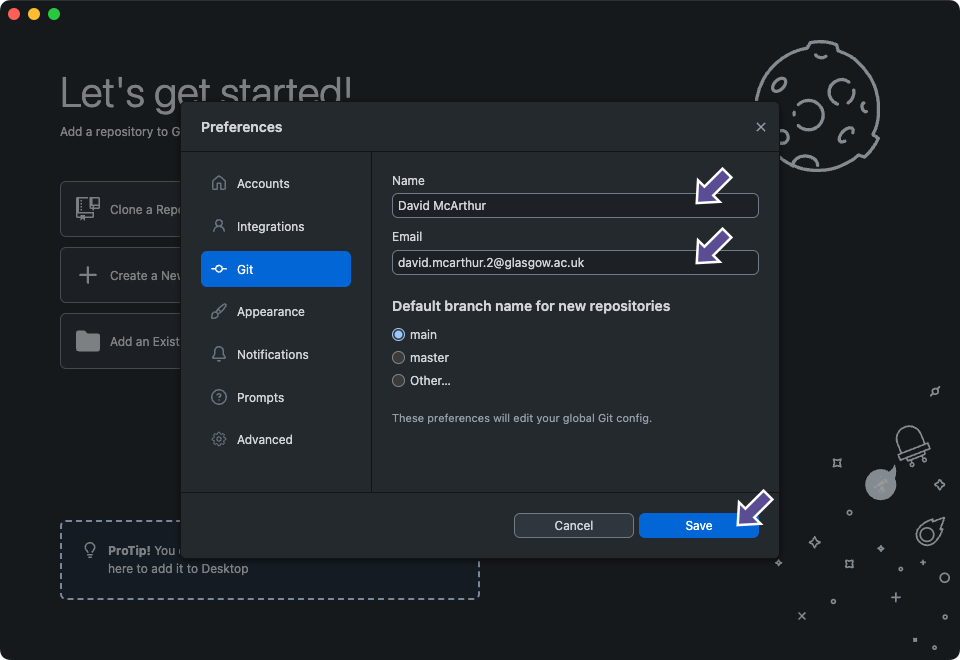
\includegraphics{images/image4.png}

\section{Connect to GitHub}\label{connect-to-github}

Let's configure Git to communicate securely with our GitHub account.

\subsection{Command-line}

The most common way to seamlessly and securely connect Git to GitHub is
using SSH (Secure Shell Protocol). If you are unfamiliar with the
concepts and workflow of SSH, be prepared to spend a little time
learning how it works and setting it up. Thankfully GitHub has excellent
documentation for Mac, Windows and Linux on this subject which is
provided below.

The process is as follows:

\subsubsection{Create an SSH keypair and add the private key to
ssh-agent}\label{create-an-ssh-keypair-and-add-the-private-key-to-ssh-agent}

First, run a command which generates an SSH key pair--- a public key and
a private key. When prompted, enter a passphrase of your choice. Next,
add the private key and associated passphrase to ssh-agent.

Full instructions can be found on GitHub for
\href{https://docs.github.com/en/authentication/connecting-to-github-with-ssh/generating-a-new-ssh-key-and-adding-it-to-the-ssh-agent}{generating
a new SSH key and adding it to the ssh-agent}.

\subsubsection{Add the public key to your account on
GitHub}\label{add-the-public-key-to-your-account-on-github}

Full instructions can be found on GitHub for
\href{https://docs.github.com/en/authentication/connecting-to-github-with-ssh/adding-a-new-ssh-key-to-your-github-account}{adding
a new SSH key to your GitHub account}.

\subsubsection{Test the connection}\label{test-the-connection}

You can test the connection by running the command:

\begin{Shaded}
\begin{Highlighting}[]
\NormalTok{ ssh }\SpecialCharTok{{-}}\NormalTok{T git}\SpecialCharTok{@}\NormalTok{github.com}
\end{Highlighting}
\end{Shaded}

Full instructions can be found on GitHub for
\href{https://docs.github.com/en/authentication/connecting-to-github-with-ssh/testing-your-ssh-connection}{testing
your SSH connection}.

\subsection{GitHub Desktop}

From the main menu, select GitHub
\texttt{Desktop\ \textgreater{}\ Settings...}. In the settings pane,
select `Accounts' from the sidebar, and click the `Sign In' button
underneath `GitHub.com':

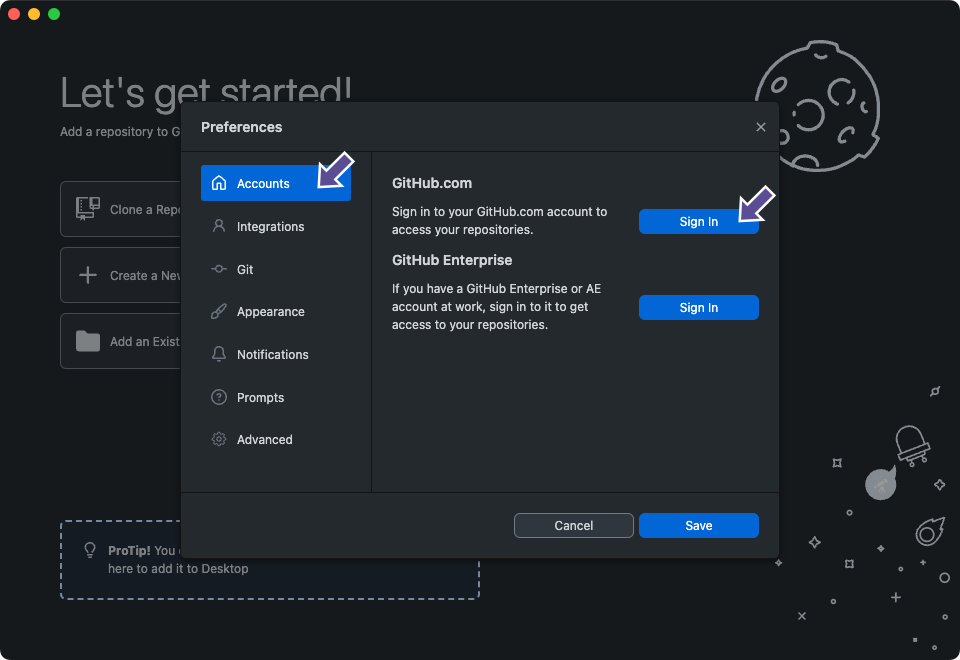
\includegraphics{images/image5.png}

\section{Set your preferred code
editor}\label{set-your-preferred-code-editor}

Lastly, As part of using Git/GitHub you often need to write short
messages explaining the changes you have made, which are often useful
when others (or indeed yourself a few months down the line) are looking
at your project.

Thus it is useful to set the preferred application that you might want
to use for this task.

\subsection{Command-line}

When you create a Git commit, which you will do often, Git will ask you
to write a message and open \href{https://www.vim.org}{Vim} by default.
Vim is a very powerful terminal-based code editor, with complicated
commands which makes some tasks when editing text or code much easier.
However, Vim has a (famously) steep learning curve, and it is out of
scope for this course however there are some excellent resources online
if you wish to learn more.

If you are not familiar with Vim you could swap to an alternative editor
(see the next few sections), although this change will only affect
certain operations (e.g.~writing a commit message if you did not specify
it on the command line), and for other operations you will need to basic
Vim, which we will introduce when appropriate.

If you do decide to use Vim or alternatively accidentally start it,
slightly infuriatingly, for those who have not worked with it before, it
is not easy to close! Hint: press : then q.

\subsubsection{Nano}\label{nano}

Nano is a popular choice when changing Vim, as even if it is unfamiliar
to you, it's still command-line-based, and much more intuitive as it has
helpful instructions at the bottom of each screen.

\begin{figure}[H]

{\centering 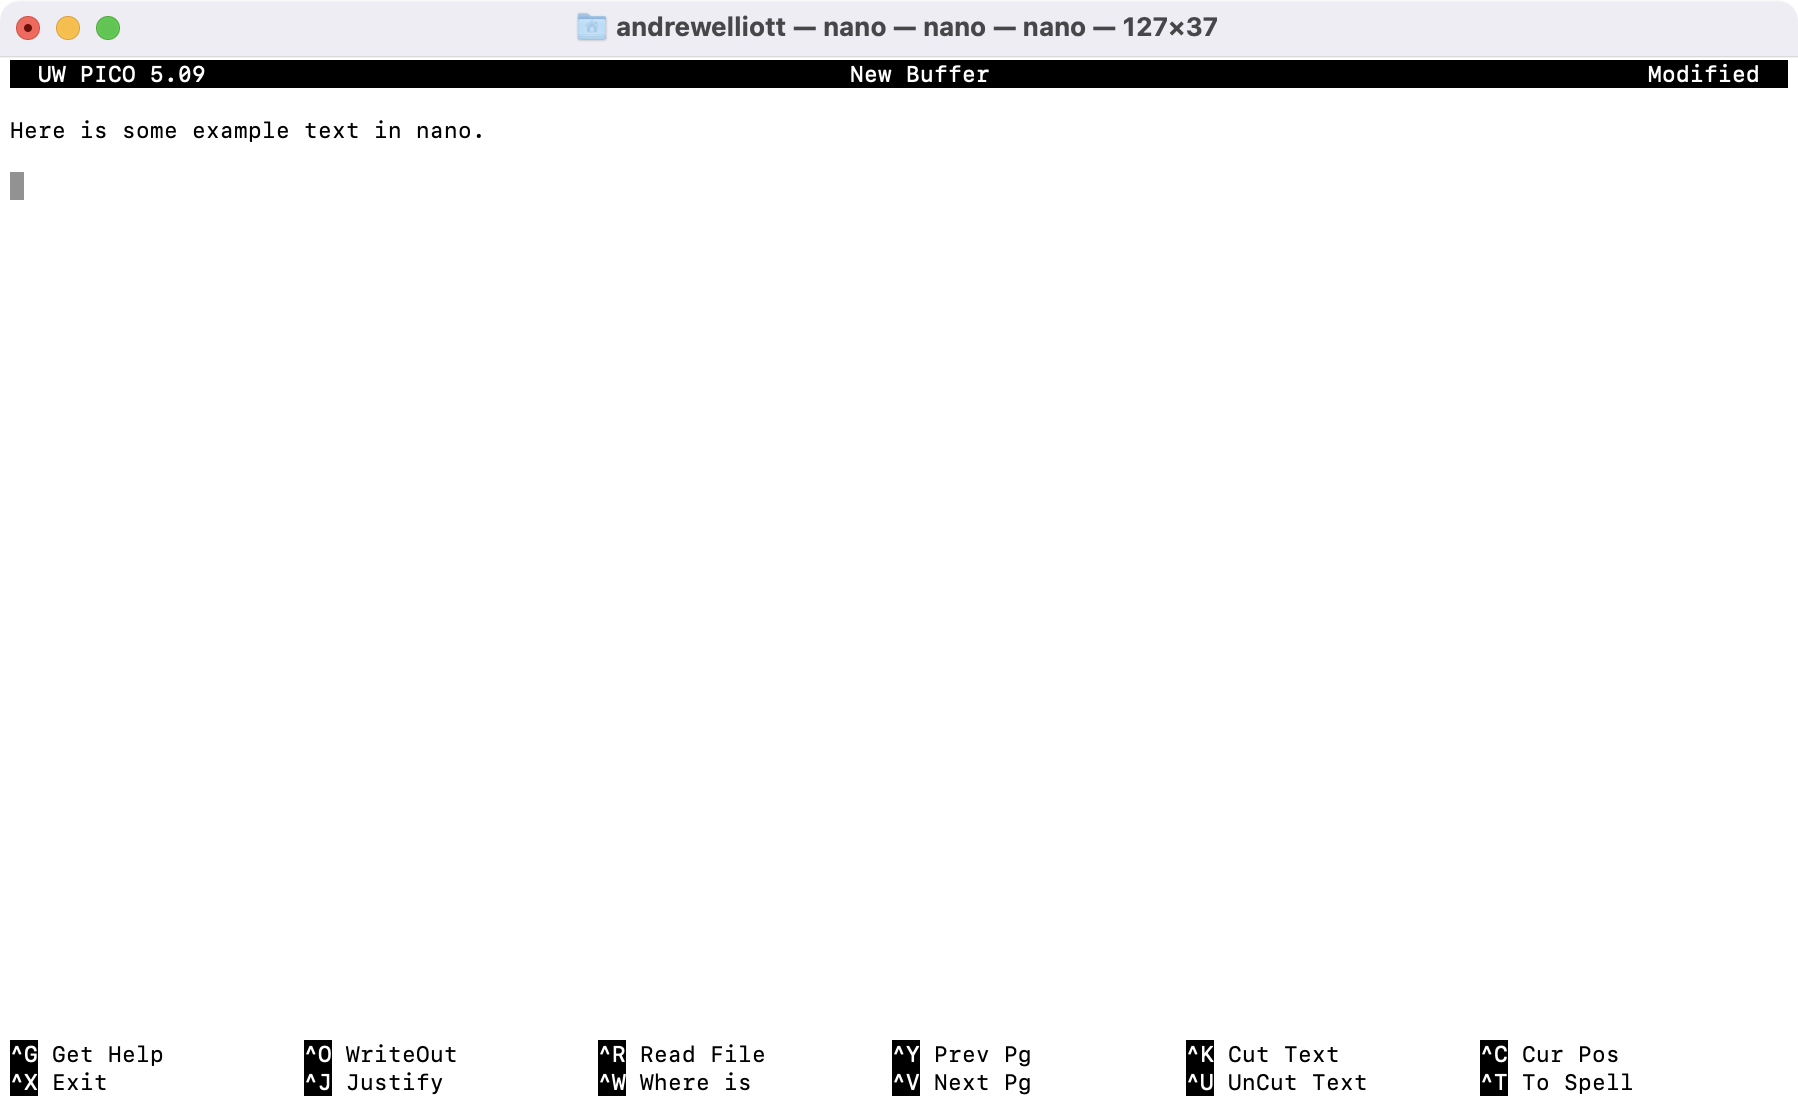
\includegraphics{images/image6.png}

}

\caption{An example of a Nano window}

\end{figure}%

To change Git's editor to Nano use the following command:

\begin{Shaded}
\begin{Highlighting}[]
\NormalTok{git config }\SpecialCharTok{{-}{-}}\NormalTok{global core.editor }\StringTok{"nano"}
\end{Highlighting}
\end{Shaded}

\subsubsection{Other editors}\label{other-editors}

Most code editors can be configured to open via the command line. The
first step is to ensure your preferred editor can be opened this way,
for example:

\begin{itemize}
\item
  \href{https://code.visualstudio.com}{VSCode} can be opened with
  \texttt{code} after
  \href{https://stackoverflow.com/questions/29955500/code-not-working-in-command-line-for-visual-studio-code-on-osx-mac}{running
  a script}.
\item
  \href{https://www.sublimetext.com}{Sublime Text} can be opened with
  \texttt{subl} after
  \href{https://stackoverflow.com/questions/25152711/subl-command-not-working-command-not-found/25154529}{running
  a script}.
\item
  \href{https://rstudio.com/products/rstudio}{RStudio} can be opened
  with \texttt{rs}
  \href{https://www.xiegerts.com/post/open-rstudio-from-terminal/}{after
  running a script}.
\end{itemize}

Once this is tested and working for your preferred editor, you can tell
Git to use this command. Some editors also require a --wait flag, or
they will open a blank page. For example:

\begin{Shaded}
\begin{Highlighting}[]
\NormalTok{git config }\SpecialCharTok{{-}{-}}\NormalTok{global core.editor }\StringTok{"subl {-}{-}wait"}
\end{Highlighting}
\end{Shaded}

\subsection{GitHub Desktop}

From the main menu, select GitHub
\texttt{Desktop\ \textgreater{}\ Settings...}. In the settings pane,
select `Integrations', then select your preferred code editor from the
dropdown under `External Editor':

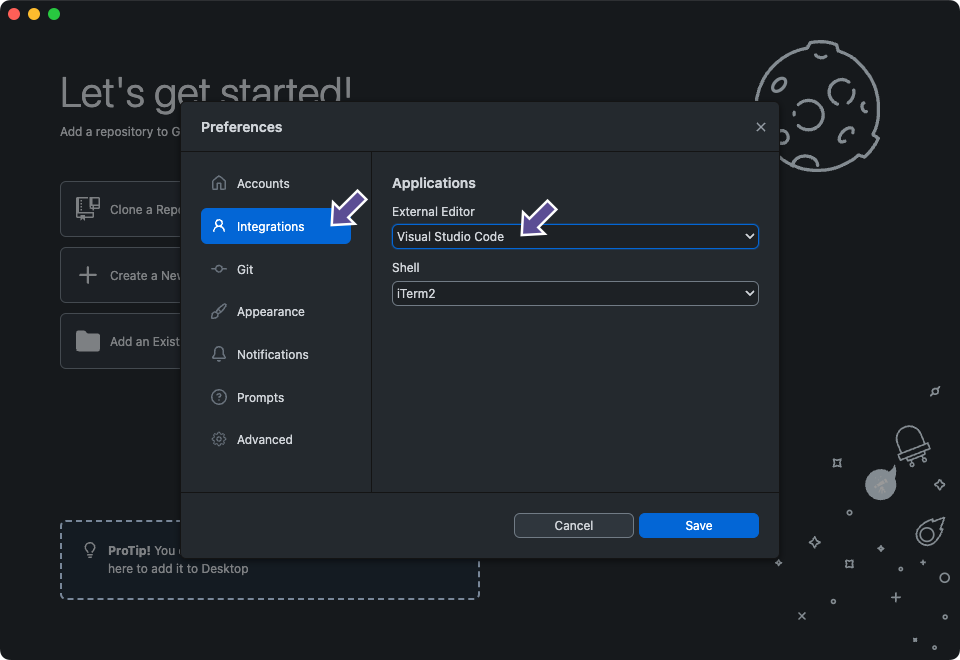
\includegraphics{images/image7.png}

\section{Basic workflow for a single
user}\label{basic-workflow-for-a-single-user}

This section aims to familiarise you with Git commands, and the Git
ethos. If you are using Git and GitHub primarily as a backup and sharing
tool, then this section is for you. You may find more technically
accurate descriptions of these commands elsewhere online, but in this
tutorial, we will aim to minimise jargon as much as possible to ease
understanding, particularly for those of you without a Computing Science
background.

To illustrate some of the concepts behind git and GitHub we will use a
graphical approach using a Git visualisation library called gitgraph.
This will allow us to give a graphical understanding of what git is
doing, alongside showing how to do this with either the command line or
GitHub Desktop. These visualisations will be very important when we
explore branching.

\subsection{Process Outline}\label{process-outline}

One way to think about a Git/GitHub project is a folder on your local
computer which is version controlled and potentially (also) on GitHub.

To set up this structure, the workflow we are going to look at next is
creating a local project folder, adding a file, initialising Git, and
then saving a copy to Github. It's also a valid workflow to first create
a GitHub repository, then `clone' it to your computer (see Unit 3).

As part of this course, you can either follow the instructions for
Command-line or GitHub Desktop. Simply choose the tab you want below and
all sections will change to the desired format. For example, the outline
of the workflow is different for the two options, as GitHub Desktop
automates some of the tasks:

\subsection{Command-line}

\begin{enumerate}
\def\labelenumi{\arabic{enumi}.}
\item
  Create a local repository
\item
  Create a new file
\item
  Add the file to the Git `stage'
\item
  Commit the file
\item
  Create a new repository on GitHub
\item
  Configure our local repository to point to the new GitHub repository
  as a remote `origin'
\item
  Push our commit(s) to sync them with the repository on GitHub.
\end{enumerate}

\subsection{GitHub Desktop}

\begin{enumerate}
\def\labelenumi{\arabic{enumi}.}
\item
  Create a local repository
\item
  Create a file
\item
  Commit the file
\item
  Publish the repository on GitHub.
\end{enumerate}

Finally, we are going to look at how you update this file. This
essentially follows the same process where we:

\begin{enumerate}
\def\labelenumi{\arabic{enumi}.}
\item
  Update the file (or add one)
\item
  Add the changes
\item
  Commit the changes
\item
  Push the changes
\end{enumerate}

\subsection{Create a local Git repository}\label{sec-local_git}

First we need to create a local Git repository which will allow us to
work through this tutorial. Ensure you have Git installed (see the
`Installation and command-line usage' section).

\subsection{Command-line}

Create an empty folder on your computer using \texttt{mkdir} and then
change to that directory using \texttt{cd}:

\begin{Shaded}
\begin{Highlighting}[]
\NormalTok{mkdir tutorial1}
\end{Highlighting}
\end{Shaded}

Alternatively as we will create several tutorials throughout this course
you may wish to first create a folder to contain them and then create
the folder for the first tutorial.

Then run \texttt{git\ init} to initialise Git inside the folder:

\begin{Shaded}
\begin{Highlighting}[]
\NormalTok{cd tutorial1}
\NormalTok{git init}
\end{Highlighting}
\end{Shaded}

\begin{verbatim}
Initialized empty Git repository in /Users/staff/Work/tutorial1/.git/
\end{verbatim}

The \texttt{git\ init} command turns a simple folder into a Git
repository.

\subsection{GitHub Desktop}

Choose \texttt{File\ \textgreater{}\ New\ Repository...} from the menu.

In the ``Create a New Repository'' form, name the repository
``tutorial1'', set the ``Local Path'' field to your preferred location
and click the ``Create Repository'' button:

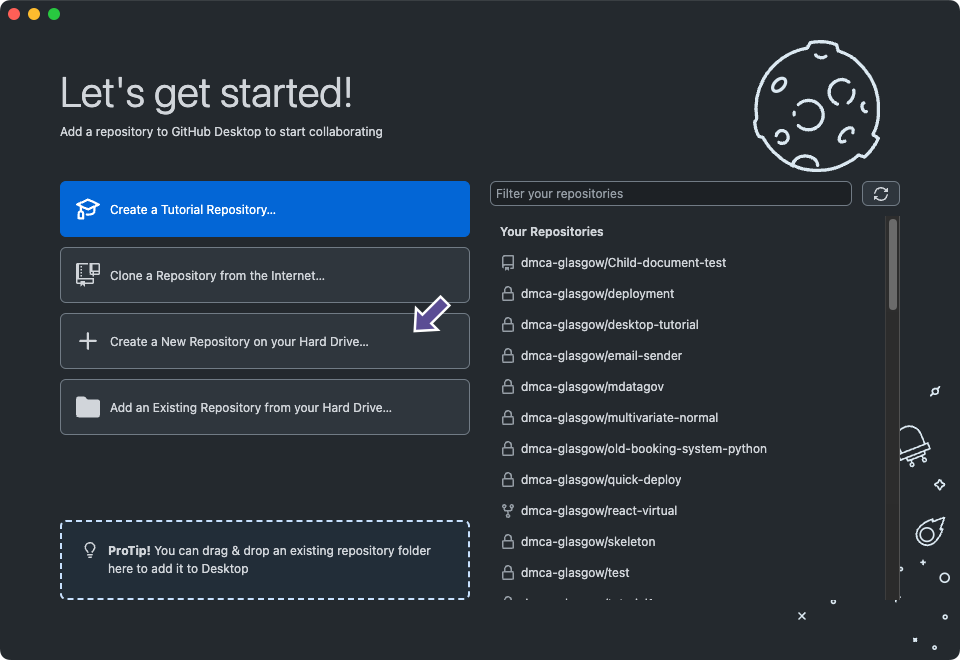
\includegraphics{images/image8.png}

That's it! You now have a local Git repository running in this folder.
We will come back and learn more about the settings for the README, Git
Ignore, and License later on in the course. We can now visualise our new
git repository, however as we have not added anything to our git it is
currently empty.

Git has created a new folder inside your folder called \texttt{.git}.
You may not be able to see this folder on a Mac or Windows operating
system, as it is a convention for files and folders that start with a
\texttt{.} to be hidden by default. However, it is important to know
that the folder is there, as it holds information that is necessary for
Git to function correctly. This folder should not be manually edited,
instead, you should use Git commands which in turn update the
information here. If you decide to move all your files to another folder
for some reason, be careful to also move this .git folder if you want to
keep using your Git repository!

In the Finder on MacOS you can show hidden files using the following
keyboard shortcut:

\begin{Shaded}
\begin{Highlighting}[]
\NormalTok{Shift }\SpecialCharTok{+}\NormalTok{ Command }\SpecialCharTok{+} \StringTok{"."}
\end{Highlighting}
\end{Shaded}

In File Explorer on Windows, select:

\begin{Shaded}
\begin{Highlighting}[]
\NormalTok{View }\SpecialCharTok{\textgreater{}}\NormalTok{ Show }\SpecialCharTok{\textgreater{}}\NormalTok{ Hidden items.}
\end{Highlighting}
\end{Shaded}

\subsection{Create a file}\label{create-a-file}

Now let's add a file. Of course, this would usually be code,
configuration, or documentation files, but to keep this course somewhat
generic and avoid distracting programming concepts, let's add a short
poem in a plain text file \texttt{poem.txt} to the folder.

You should use your preferred Code Editor to create the file, such as
VSCode or RStudio. If using Word or other ``rich text'' editors ensure
you choose the File Format ``Plain text (\texttt{.txt})'' when saving
the file.

\begin{Shaded}
\begin{Highlighting}[]
\NormalTok{Now We Are Six by A. A. Milne}

\NormalTok{When I was One,}
\NormalTok{I had just begun.}
\NormalTok{When I was Two,}
\NormalTok{I was nearly new.}
\NormalTok{When I was Three}
\NormalTok{I was hardly me.}
\NormalTok{When I was Four,}
\NormalTok{I was not much more.}
\NormalTok{When I was Five,}
\NormalTok{I was just alive.}
\NormalTok{But now I am Six,}
\NormalTok{I\textquotesingle{}m as clever as clever,}
\NormalTok{So I think I\textquotesingle{}ll be six now for ever and ever.}
\end{Highlighting}
\end{Shaded}

Ensure the file is saved in your local repository. Git can only `see'
changes that are saved.

\subsection{Git status}\label{git-status}

\subsection{Command-line}

Let's have our first look at the output of
\texttt{git\ status}.\texttt{git\ status} tries to provide helpful
information depending on your current situation.

When using Git, you'll run git status so often that it will soon become
muscle memory! The \texttt{git\ status} command only outputs status
information and won't modify commits or changes in your local
repository.

Now we've created a file let's see what it outputs:

\begin{Shaded}
\begin{Highlighting}[]
\NormalTok{git status}
\end{Highlighting}
\end{Shaded}

\begin{verbatim}
On branch main

No commits yet

Untracked files:
(use "git add <file>..." to include in what will be committed)
poem.txt

nothing added to commit but untracked files present (use "git add" to track)
\end{verbatim}

\begin{enumerate}
\def\labelenumi{\arabic{enumi}.}
\item
  We can see that Git knows we're on the main branch (we'll introduce
  branching concepts gradually as we progress through the course).
\item
  There have been no commits yet (more on this later in this unit).
\item
  Git knows our \texttt{poem.txt} file has been created but it is still
  ``untracked'' (a version has not been explicitly added to Git yet and
  therefore this file is not covered by version control)
\end{enumerate}

The \texttt{-\/-short} or \texttt{-s} flag removes all but the most
relevant information:

\begin{Shaded}
\begin{Highlighting}[]
\NormalTok{git status }\SpecialCharTok{{-}}\NormalTok{s}
\end{Highlighting}
\end{Shaded}

\begin{verbatim}
?? poem.txt
\end{verbatim}

Here we can see the Git shortened syntax for ``untracked'' is ??.

\subsection{GitHub Desktop}

Let's have a look at GitHub Desktop. As you work on your project GitHub
Desktop will watch your files update when it detects changes:

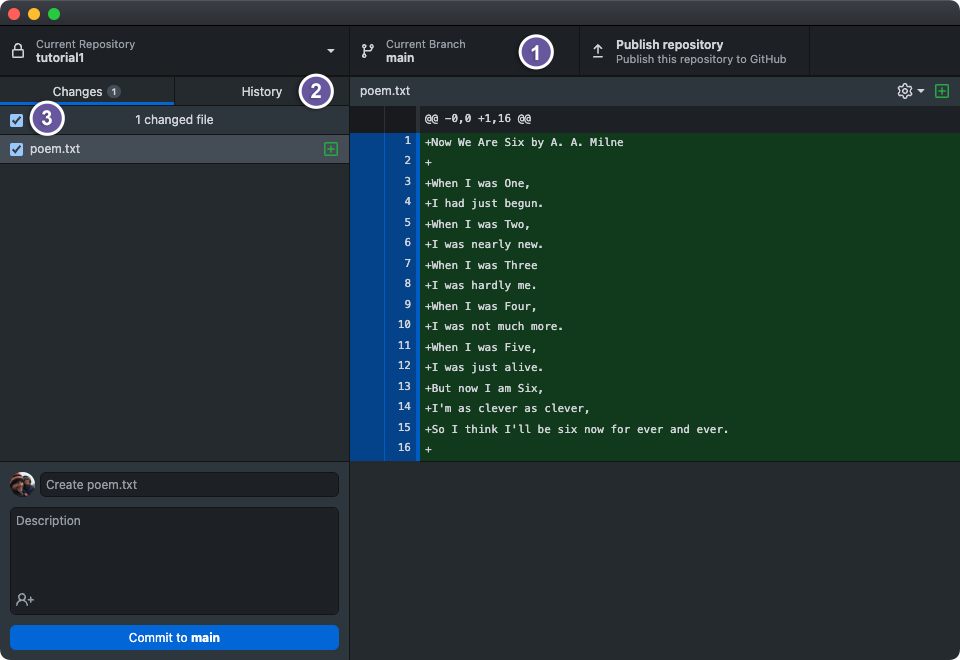
\includegraphics{images/image9.png}

Here we can see Git has found our new file! We have added some numbered
purple circles to the screenshot above, let's go through those areas:

\begin{enumerate}
\def\labelenumi{\arabic{enumi}.}
\item
  Here we can see that Git knows we're on the main branch (we'll
  introduce branching concepts gradually as we progress through the
  course).
\item
  If you click on the History tab, you'll see there have been no commits
  yet (more on this later in this unit).
\item
  The checkbox beside the filename is checked, which in Git terms, means
  the file has been ``staged'' for commit
\end{enumerate}

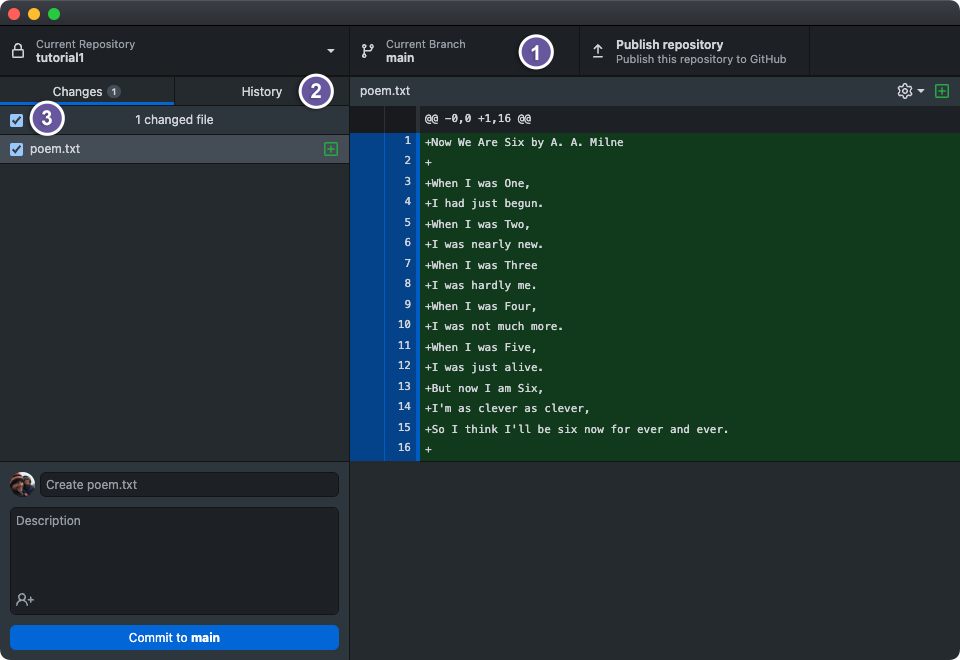
\includegraphics{images/image9.png}

\subsection{Adding our file to our
project}\label{adding-our-file-to-our-project}

\subsubsection{Stage the file}\label{stage-the-file}

Adding files to the stage is an intermediate step before committing to a
version. We need to choose (stage) the files we want to add to our
commit. Staging may seem an unnecessary step at this point, but later we
will demonstrate how this can be a powerful tool.

For now, we will stage all changes, our only file poem.txt.

\subsection{Command-line}

We can stage the file using the add command:

\begin{Shaded}
\begin{Highlighting}[]
\NormalTok{git add poem.txt}
\end{Highlighting}
\end{Shaded}

Note that there two options here: *
\texttt{git\ add\ \textless{}path\textgreater{}}: Stage a specific
directory or file * \texttt{git\ add\ .}: Stage all files (that are not
listed in the .gitignore) in the entire repository.

Now we've staged the file let's have a look at the status again:

\begin{Shaded}
\begin{Highlighting}[]
\NormalTok{git status}
\end{Highlighting}
\end{Shaded}

\begin{verbatim}
On branch main

No commits yet

Changes to be committed:
(use "git rm --cached <file>..." to unstage)
new file:   poem.txt
\end{verbatim}

Our \texttt{poem.txt} file has been added to the stage! If we view the
short version we can see \texttt{A} for ``add'':

\begin{Shaded}
\begin{Highlighting}[]
\NormalTok{git status }\SpecialCharTok{{-}}\NormalTok{s}
\end{Highlighting}
\end{Shaded}

\begin{verbatim}
A  poem.txt
\end{verbatim}

There is also a \texttt{-\/-verbose} or \texttt{-v} flag. In this case,
it also includes the ``diff'' of \texttt{poem.txt} (more information on
what a ``diff'' is after this example):

\begin{Shaded}
\begin{Highlighting}[]
\NormalTok{git status }\SpecialCharTok{{-}{-}}\NormalTok{verbose}
\end{Highlighting}
\end{Shaded}

\begin{verbatim}
On branch main

No commits yet

Changes to be committed:
(use "git rm --cached <file>..." to unstage)
new file:   poem.txt

diff --git a/poem.txt b/poem.txt
new file mode 100644
index 0000000..12f4ac3
--- /dev/null
+++ b/poem.txt
@@ -0,0 +1,16 @@
+Now We Are Six by A. A. Milne
+
+When I was One,
+I had just begun.
+When I was Two,
+I was nearly new.
+When I was Three
+I was hardly me.
+When I was Four,
+I was not much more.
+When I was Five,
+I was just alive.
+But now I am Six,
+I'm as clever as clever,
+So I think I'll be six now for ever and ever.
+
\end{verbatim}

We can view this ``diff'' output on its own using the command in the
next box.

\subsection{GitHub Desktop}

\begin{enumerate}
\def\labelenumi{\arabic{enumi}.}
\tightlist
\item
  GitHub Desktop has automatically added our new file to the stage as
  you can see by the checked checkbox.
\item
  The green plus symbol here indicates this is a new file (or
  technically, it has not been added to Git yet).
\item
  This area displays the ``diff'' of \texttt{poem.txt} (more information
  on what a ``diff'' is after this example).
\end{enumerate}

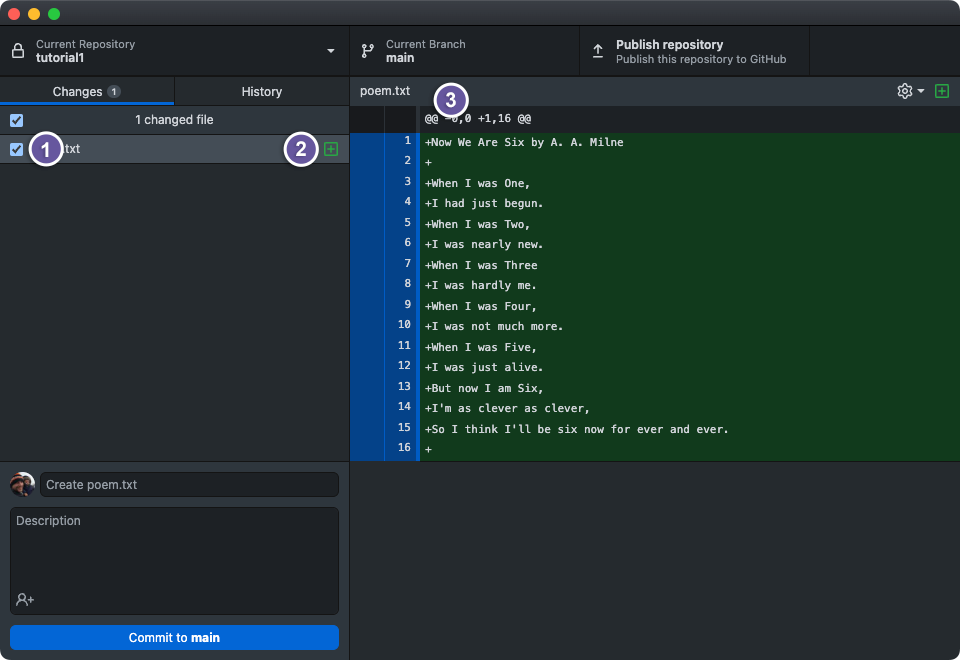
\includegraphics{images/image10.png}

\subsubsection{Commit the first version}\label{commit-the-first-version}

Once we have determined which files we want to stage, we can then commit
the change(s). Importantly unlike (say) Dropbox, the changes in your
project are not stored until you tell Git that they are ready to be
stored i.e.~in Git you `commit' them.

The act of `committing' in Git creates a `version' (sometimes just
called a `commit'). A version can be thought of as a snapshot of your
whole project at that time. Once a commit has been made, it's always
possible to get back to this version. This simple concept can be
extremely powerful for the evolution and maintenance of small to very
large programming projects.

Each version should be accompanied by a message describing the change
made by the commit. This can be a skill in itself as you wish to tell
your collaborators or your future self what changes have been made (we
will discuss best practices in Unit 4).

\subsection{Command-line}

Now let's create our first commit!

\begin{Shaded}
\begin{Highlighting}[]
\NormalTok{git commit }\SpecialCharTok{{-}{-}}\NormalTok{message }\StringTok{"Create poem.txt"}
\end{Highlighting}
\end{Shaded}

\begin{verbatim}
[main (root-commit) acf18e1] Create poem.txt
1 file changed, 16 insertions(+)
create mode 100644 poem.txt
\end{verbatim}

If you do not specify a message then Git will open up your text editor
of choice (see unit 1) to add a message.

Experienced users will use the shorthand \texttt{-m} instead of
\texttt{-\/-message}, i.e.~\texttt{git\ commit\ -m\ "Create\ poem.txt"}.

Git status shows ``working tree clean'', which means all changes
detected in the directory have been committed to Git:

\begin{Shaded}
\begin{Highlighting}[]
\NormalTok{git status}
\end{Highlighting}
\end{Shaded}

\begin{verbatim}
On branch main
nothing to commit, working tree clean
\end{verbatim}

Let's have our first look at the log:

\begin{Shaded}
\begin{Highlighting}[]
\NormalTok{git log}
\end{Highlighting}
\end{Shaded}

\begin{verbatim}
commit acf18e19f0803fd405f7d1e196fbaf710066728d
Author: David McArthur <david.mcarthur.2@glasgow.ac.uk>
Date:   Mon Aug 21 13:41:25 2023 +0100

Create poem.txt
\end{verbatim}

There is a log of our first version! (Again this opens vim, and to exit
press \texttt{:} followed by \texttt{q}).

\subsection{GitHub Desktop}

Make sure the file is staged making sure the checkbox \texttt{poem.txt}
is ticked, add the message ``Create poem.txt'' to the summary, then
click the ``Commit to main'' button:

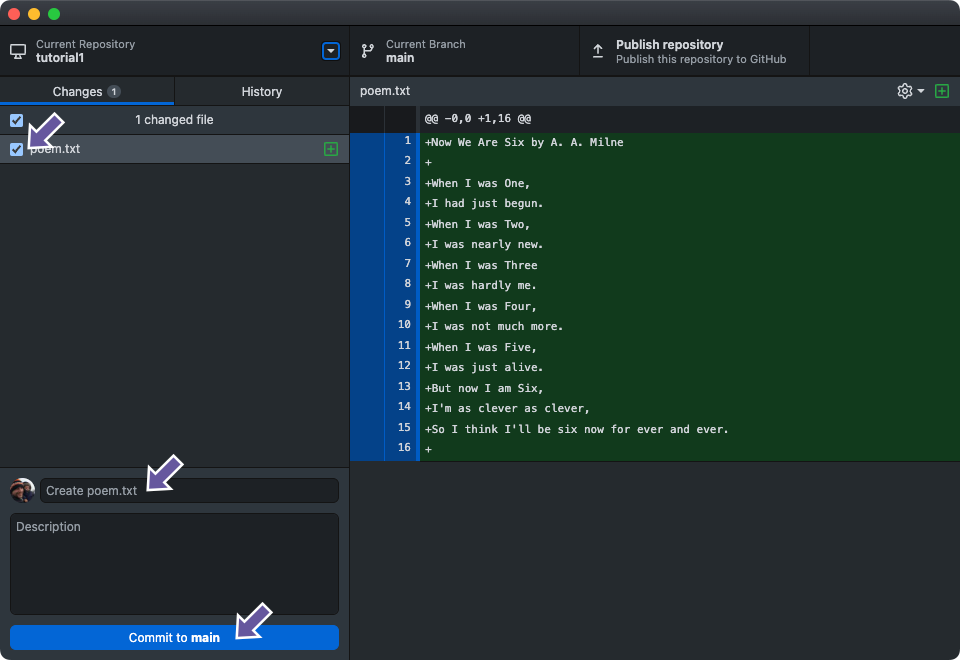
\includegraphics{images/image11.png}

We have created our first commit! GitHub Desktop now says we have ``No
local changes'', which means all changes detected in the directory have
been committed to Git:

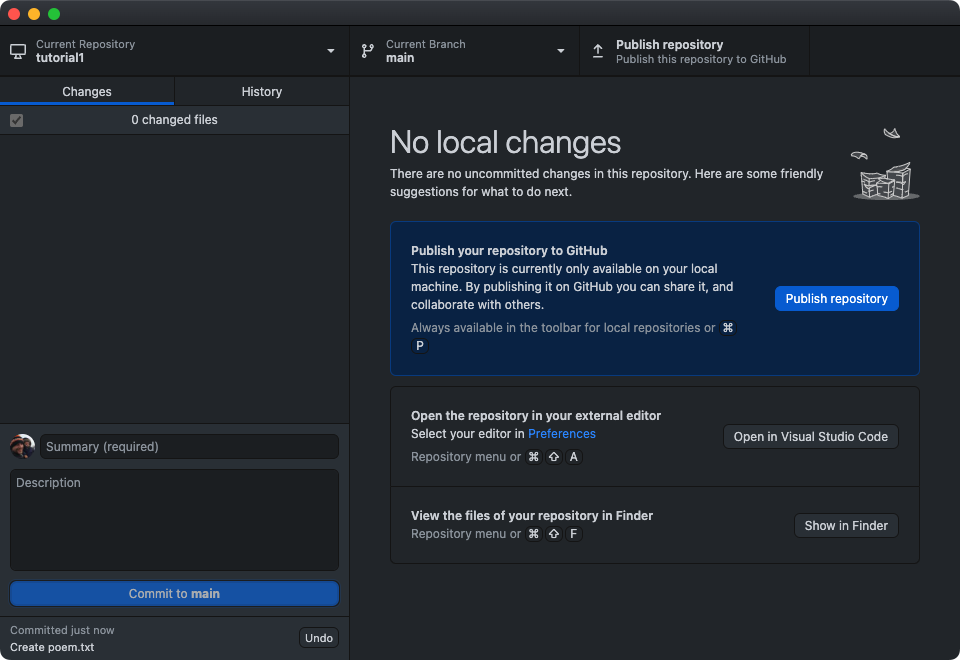
\includegraphics{images/image12.png}

Where did our commit go? By clicking on the ``History'' tab, we can see
our first commit:

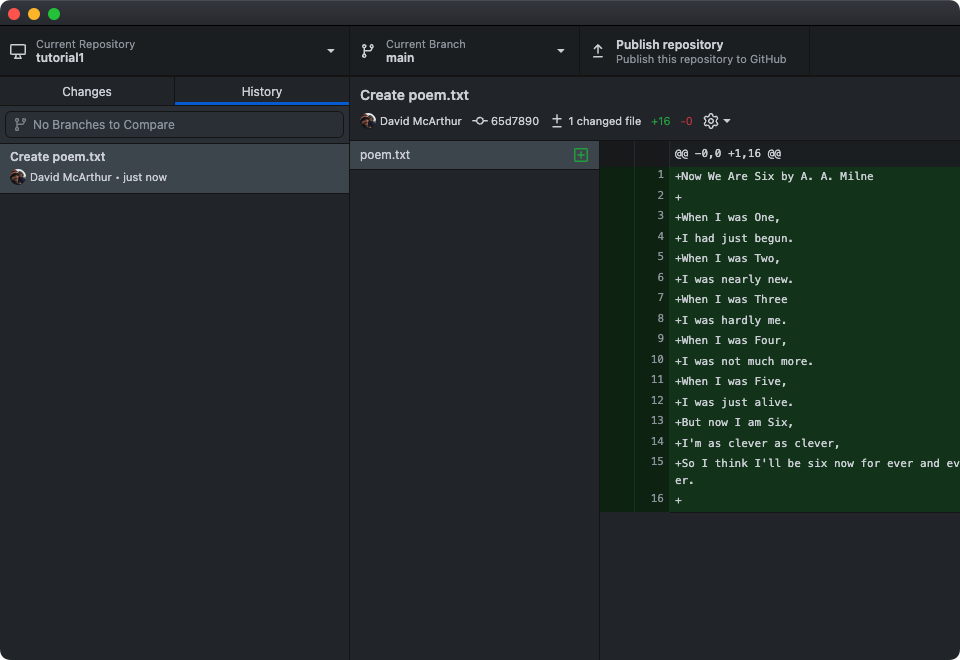
\includegraphics{images/image13.png}

\subsection{Get our project onto
GitHub}\label{get-our-project-onto-github}

You have now created a Git repository on your local machine and added a
file, however this is only available to people who use your computer. In
this section we will demonstrate how to make this available to everyone
via the GitHub website.

\subsubsection{Create a new repository on
GitHub}\label{create-a-new-repository-on-github}

Up to this point, we have been using Git locally. Next, let's learn how
to put a copy of our project on GitHub to share it with others or just
make a backup for ourselves.

\begin{tcolorbox}[enhanced jigsaw, left=2mm, breakable, toptitle=1mm, colback=white, coltitle=black, opacitybacktitle=0.6, leftrule=.75mm, colbacktitle=quarto-callout-caution-color!10!white, rightrule=.15mm, bottomrule=.15mm, bottomtitle=1mm, titlerule=0mm, title=\textcolor{quarto-callout-caution-color}{\faFire}\hspace{0.5em}{\textbf{Private or Public Repository}}, colframe=quarto-callout-caution-color-frame, opacityback=0, arc=.35mm, toprule=.15mm]

When creating a GitHub repository, you will need to decide if it will be
private or public. Private will mean the code is only available to
yourself and other contributors, but public will mean that anyone will
be able to see your code. The purpose and stage of your project will
determine which of these makes the most sense.

The decision is ultimately a pragmatic one, and can strongly depend on
your particular circumstances, for example, you may wish to develop a
new open-source software library in a public repository to encourage
interest and contributions from others earlier, or you may wish to keep
it private either for your own use only or until it is ready to be
shared. Approaches to this can also vary, in some parts of Academia it
is common to having a public repository on active research projects, in
others a repository is made public once the project has finished.

\textbf{Important:}~Be careful not to put anything sensitive on a public
repository as it will be accessible to all, although it is probably not
to put it on GitHub either way.

\end{tcolorbox}

\subsection{Command-line}

To be able to add our content to a GitHub page (remote repository), you
will firstly need to create a repository. GitHub Desktop does this for
you, but for the command-line, we need to do it ourselves. You can do
this by following the Create a repo quickstart guide to create a new
repository for our example. Here it is named ``tutorial1'' but you can
name it whatever you like.

The Git command for syncing local commits with GitHub is push. Let's try
it now:

\begin{Shaded}
\begin{Highlighting}[]
\NormalTok{git push}
\end{Highlighting}
\end{Shaded}

\begin{verbatim}
fatal: No configured push destination.
Either specify the URL from the command-line or configure a remote repository using

    git remote add <name> <url>

and then push using the remote name

    git push <name>
\end{verbatim}

Git is telling us we still need to configure our local repository to use
our new GitHub repository as a remote (a remote is a copy of our
repository stored in another location, in this case on GitHub). When we
ask Git to list the configured remotes there is no output:

\begin{Shaded}
\begin{Highlighting}[]
\NormalTok{git remote}
\end{Highlighting}
\end{Shaded}

\begin{verbatim}
origin
\end{verbatim}

So let's set that up now.

On GitHub, copy the URL of your empty repository:

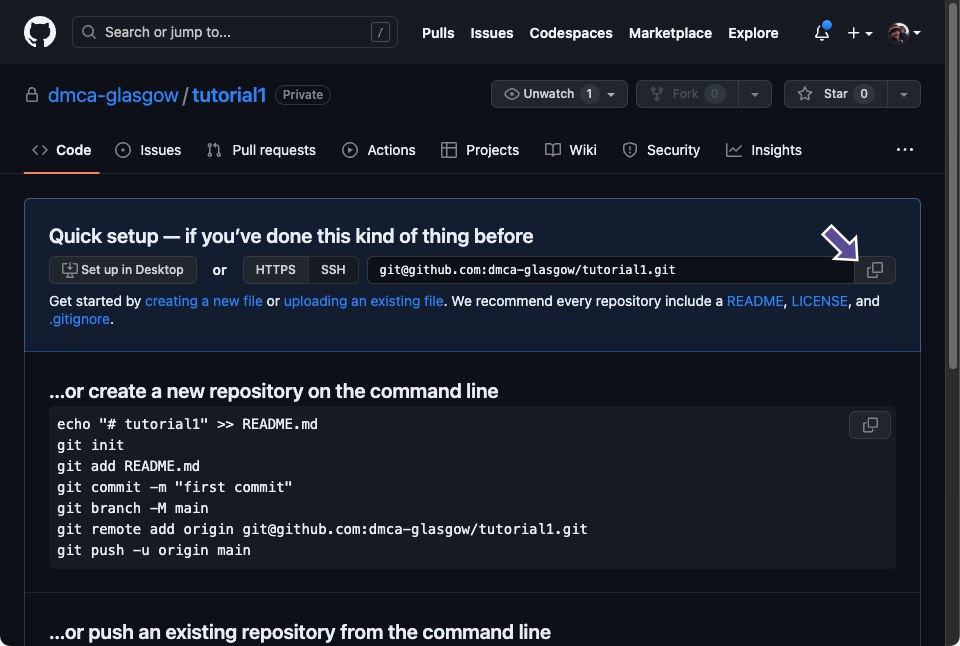
\includegraphics{images/image14.png}

And paste it in the following command:

\begin{Shaded}
\begin{Highlighting}[]
\NormalTok{git remote add origin }\SpecialCharTok{\textless{}}\NormalTok{your}\SpecialCharTok{{-}}\NormalTok{repository}\SpecialCharTok{{-}}\NormalTok{url}\SpecialCharTok{\textgreater{}}
\end{Highlighting}
\end{Shaded}

You can check \texttt{git\ remote} again:

\begin{Shaded}
\begin{Highlighting}[]
\NormalTok{git remote}
\end{Highlighting}
\end{Shaded}

\begin{verbatim}
origin
\end{verbatim}

\begin{Shaded}
\begin{Highlighting}[]
\NormalTok{git remote }\SpecialCharTok{{-}{-}}\NormalTok{verbose}
\end{Highlighting}
\end{Shaded}

\begin{verbatim}
origin  https://github.com/dmca-glasgow/tutorial1.git (fetch)
origin  https://github.com/dmca-glasgow/tutorial1.git (push)
\end{verbatim}

We can see that our GitHub repository is configured for both fetch and
push commands.

Now let's try to push again:

\begin{Shaded}
\begin{Highlighting}[]
\NormalTok{git push}
\end{Highlighting}
\end{Shaded}

\begin{verbatim}
fatal: The current branch main has no upstream branch.
To push the current branch and set the remote as upstream, use

    git push --set-upstream origin main

To have this happen automatically for branches without a tracking
upstream, see 'push.autoSetupRemote' in 'git help config'.
\end{verbatim}

Git is telling us it can't sync our local commits to main because GitHub
doesn't know about the main branch yet. So let's follow its instructions
to tell GitHub about this branch:

\begin{Shaded}
\begin{Highlighting}[]
\NormalTok{git push }\SpecialCharTok{{-}{-}}\NormalTok{set}\SpecialCharTok{{-}}\NormalTok{upstream origin main}
\end{Highlighting}
\end{Shaded}

\begin{verbatim}
To https://github.com/dmca-glasgow/tutorial1.git
  * [new branch]      main -> main
branch 'main' set up to track 'origin/main'.
\end{verbatim}

And now, if we refresh our GitHub repository page, we should see our
poem.txt file!

\subsection{Git-Desktop}

In GitHub Desktop, click the ``Publish repository'' tab, give it a name,
and click the ``Publish Repository'' button:

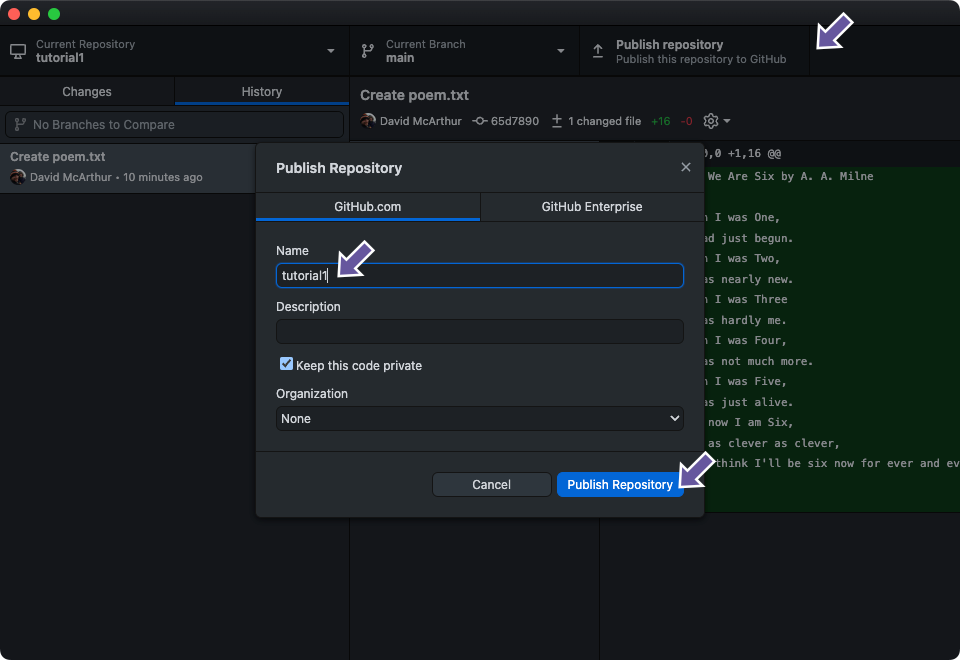
\includegraphics{images/image15.png}

And now, if we refresh our GitHub repository page, we should see our
poem.txt file!

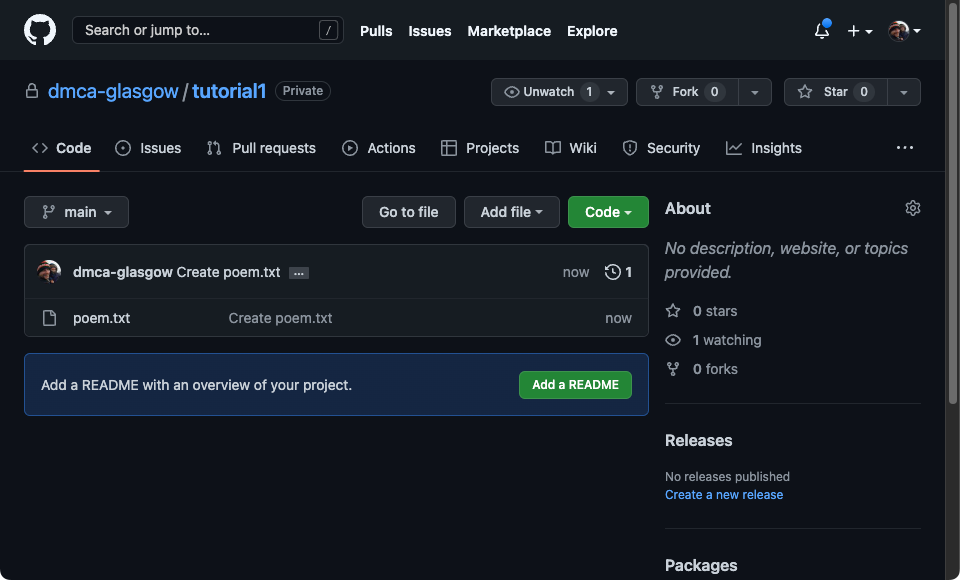
\includegraphics{images/image16.png}

We can click on the commits icon:

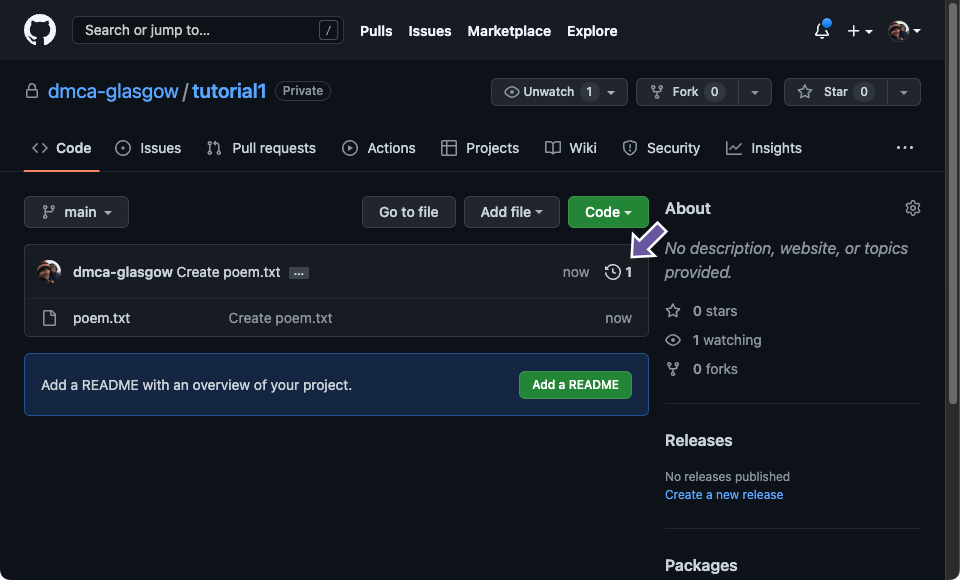
\includegraphics{images/image17.png}

To view our commit history:

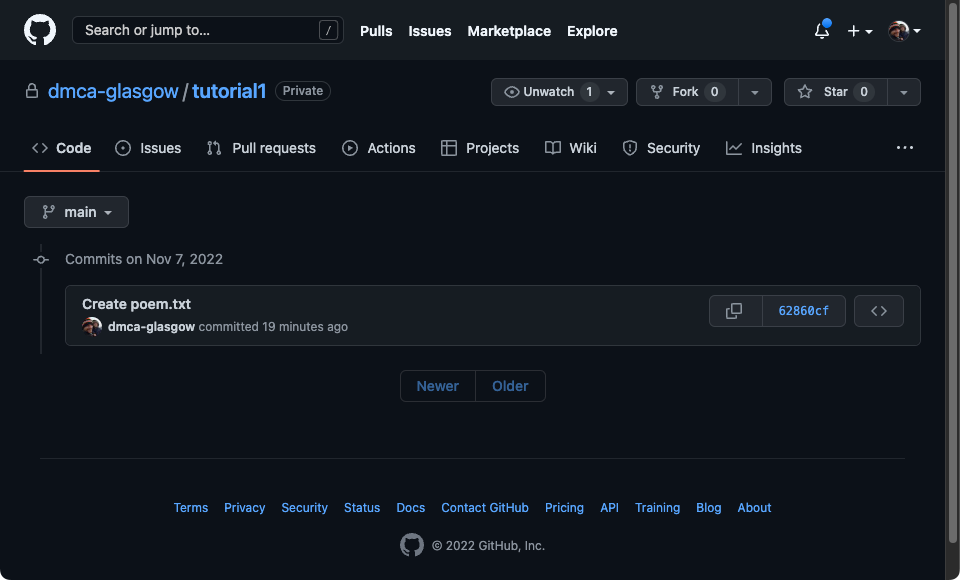
\includegraphics{images/image18.png}

And we can click on the branches button to view our main branch:

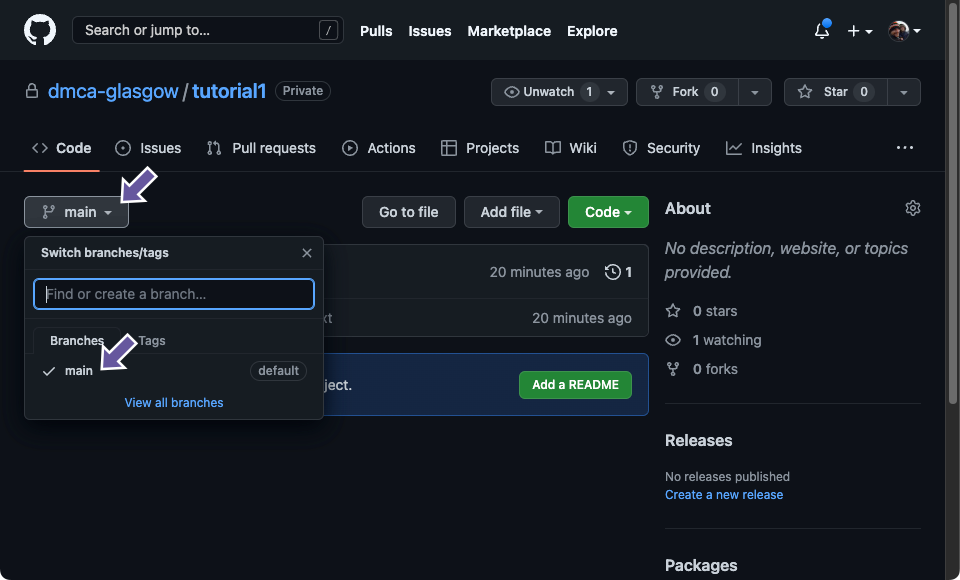
\includegraphics{images/image19.png}

\subsection{Updating your repository}\label{updating-your-repository}

Now that we have a local Git repository that is linked to GitHub, let's
briefly explore the process of updating our project.

\subsubsection{Rename the file}\label{rename-the-file}

First, let's rename our \texttt{poem.txt} file to \texttt{poem.md} (for
Markdown).

In Git terms, renaming a file is considered deleting one file
(\texttt{poem.txt}) and creating a new file (poem.md).

\subsection{Command-line}

You can see that \texttt{poem.md} currently has `untracked' status as it
has not been added to Git yet.

\begin{Shaded}
\begin{Highlighting}[]
\NormalTok{git status}
\end{Highlighting}
\end{Shaded}

\begin{verbatim}
On branch main
Your branch is up to date with 'origin/main'.

Changes not staged for commit:
(use "git add/rm <file>..." to update what will be committed)
(use "git restore <file>..." to discard changes in working directory)
deleted:    poem.txt

Untracked files:
(use "git add <file>..." to include in what will be committed)
poem.md

no changes added to commit (use "git add" and/or "git commit -a")
\end{verbatim}

\subsection{GitHub Desktop}

The icon beside \texttt{poem.md} has a plus symbol for a new, untracked
file, whereas the \texttt{poem.txt} file has a red minus symbol
indicating it has been deleted.

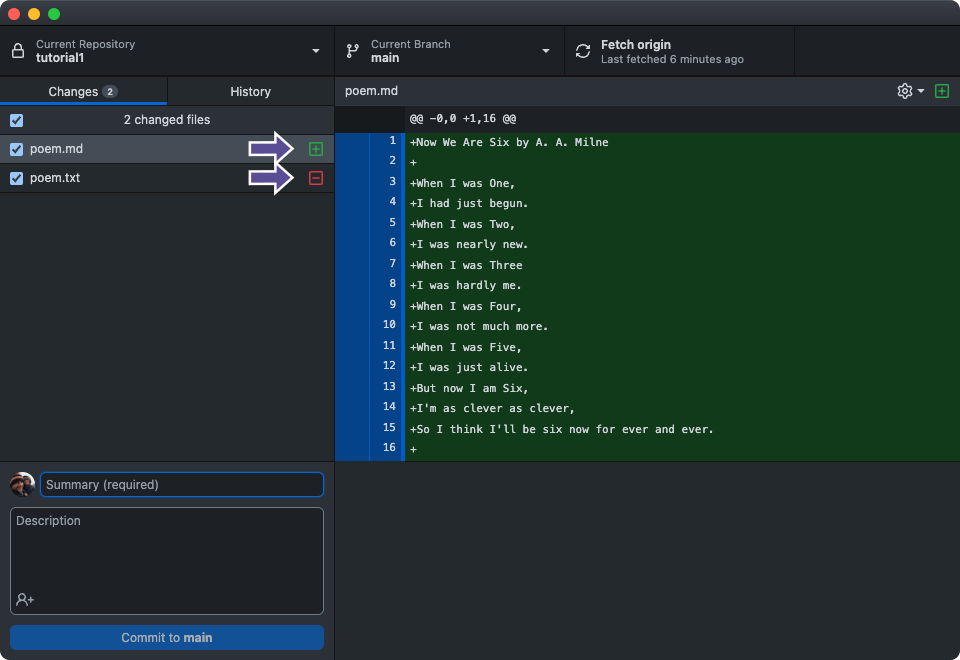
\includegraphics{images/image19_1.png}

Next, let's commit this change. It might seem counter-intuitive, but we
need to stage and commit both files in this scenario because adding a
file and deleting a file are both actions that need to be committed.

\subsection{Command-line}

Let's do that now:

\begin{Shaded}
\begin{Highlighting}[]
\NormalTok{git add poem.txt poem.md}
\end{Highlighting}
\end{Shaded}

\begin{verbatim}
git commit -m 'rename poem.txt to poem.md'
[main edac35e] rename poem.txt to poem.md
1 file changed, 0 insertions(+), 0 deletions(-)
rename poem.txt => poem.md (100%)
\end{verbatim}

\subsection{GitHub Desktop}

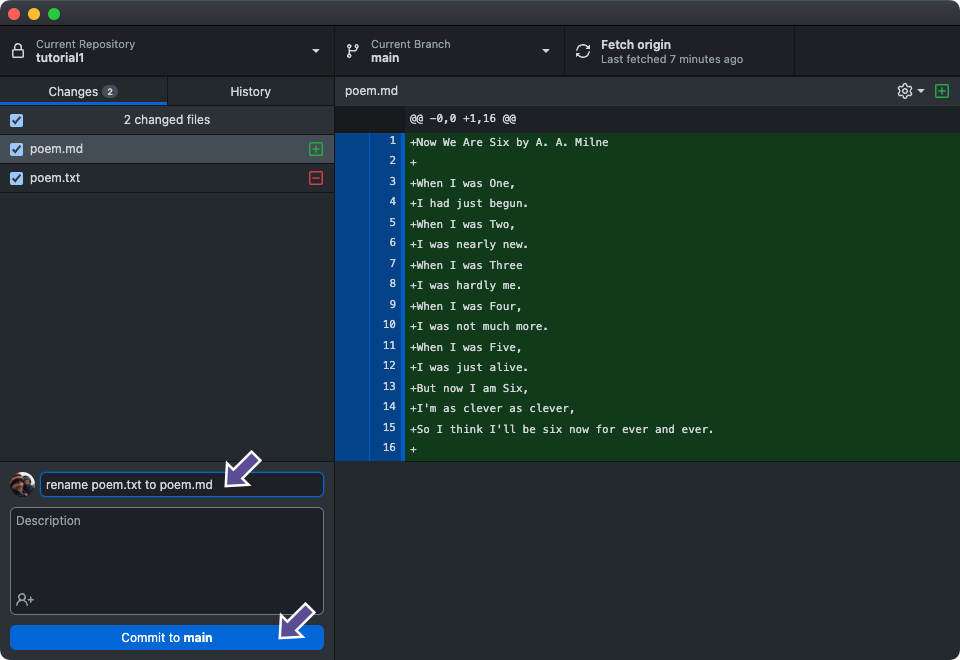
\includegraphics{images/image20.png}

\section{Supplement: Special file
conventions}\label{supplement-special-file-conventions}

Both Git and GitHub have special file conventions, where files with a
particular name have special behaviours. Git uses the `dotfile'
convention (a \texttt{.} at the start of the name), whereas GitHub
typically uses all-caps. The `dotfile' convention is relatively common
and as your operating system may know that they are used as
configuration files they may not show up in our file manager.

The most important are listed below, but please see a
\href{https://stackoverflow.com/questions/12605576\#12719247}{list of
Git special files} and a
\href{https://github.com/joelparkerhenderson/github-special-files-and-paths}{list
of GitHub special files} for more information.

\subsection{.gitignore}\label{gitignore}

When we share our codebase using Git and GitHub, either with the public
or with colleagues, we can choose to exclude certain files (e.g.~tell
Git/GitHub never to consider them) by making use of a
\texttt{.gitignore} file. To be more precise, we are telling Git to
ignore these files from our project folder by not adding them to any
commit change list.

For example:

\begin{verbatim}
# <-- comments start with a hash sign
# empty lines are ignored

# ignore 'passwords.txt' at the root of your project:
/passwords.txt

# ignore 'passwords.txt' anywhere in your project:
passwords.txt

# ignore 'cache' folder  at the root of your project:
/cache/

# ignore all 'cache' folders:
cache/

# ignore all .log files inside a 'logs' folder:
logs/*.log

# ignore all .html files inside the 'logs' folder including sub-folders:
logs/**/*.log

# ignore all files with .log extension:
**/*.log
\end{verbatim}

If a file has already been committed to Git, ignoring it with .gitignore
won't remove it from the repository, only it's changes from that point
on. If you'd like to remove a file from Git, the simplest way is to
follow these steps:

\begin{enumerate}
\def\labelenumi{\arabic{enumi}.}
\tightlist
\item
  Move the file out of your project folder
\item
  Git will treat the file as deleted. Stage and commit this change.
\item
  Add the file path to .gitignore
\item
  Move the file back into your project folder
\item
  Check the stage and confirm that Git is ignoring it
\item
  Commit the updated .gitignore file
\end{enumerate}

However, while the file has been removed it is still present in your
history in future sections.

\subsection{.gitkeep}\label{gitkeep}

A strange quirk of Git is that it is only concerned with files and not
folders. Your project can be split into as many files and folders as you
wish with no problems, but at some point, you may be confused that Git
does not `see' empty folders.

As a workaround, a common convention is to create an empty file inside
the folder named \texttt{.gitkeep}, which you can commit, enabling you
to store the (not really) empty folder in your repository.



\end{document}
